\documentclass[a4paper,ngerman,12pt]{zirkelblatt1415}

\usepackage[utf8]{inputenc}

\usepackage[ngerman]{babel}

\usepackage{amsmath,amsthm,amssymb,stmaryrd,color,graphicx}
\usepackage{setspace}
\usepackage{bussproofs}
\usepackage{array}
\usepackage{comment}

\usepackage[protrusion=true,expansion=true]{microtype}

\usepackage{lmodern}

\usepackage{hyperref}

\setlength\parskip{\medskipamount}
\setlength\parindent{0pt}

\theoremstyle{definition}
\newtheorem{defn}{Definition}[section]
\newtheorem{axiom}[defn]{Axiom}
\newtheorem{bsp}[defn]{Beispiel}

\theoremstyle{plain}
\newtheorem{prop}[defn]{Proposition}
\newtheorem{motto}[defn]{Motto}
\newtheorem{wunder}[defn]{Wunder}
\newtheorem{ueberlegung}[defn]{??berlegung}
\newtheorem{lemma}[defn]{Lemma}
\newtheorem{kor}[defn]{Korollar}
\newtheorem{hilfsaussage}[defn]{Hilfsaussage}
\newtheorem{satz}[defn]{Satz}

\theoremstyle{remark}
\newtheorem{bem}[defn]{Bemerkung}
\newtheorem{aufg}[defn]{Aufgabe}

\newcommand{\RR}{\mathbb{R}}
\newcommand{\CC}{\mathbb{C}}
\newcommand{\ZZ}{\mathbb{Z}}
\renewcommand{\NN}{\mathbb{N}}
\newcommand{\QQ}{\mathbb{Q}}
%\newcommand{\K}{\mathbb{K}}
\newcommand{\PP}{\mathbb{P}}
%\newcommand{\CP}{\mathbb{CP}}
%\newcommand{\RP}{\mathbb{RP}}
\newcommand {\kk} {\Bbbk}
\newcommand{\VV}{\mathbb V}
\newcommand{\HH}{\mathbb{H}}
\newcommand{\ii}{\mathrm{i}}
\newcommand{\AM}{\operatorname{AM}}
\newcommand{\GM}{\operatorname{GM}}
\newcommand{\HM}{\operatorname{HM}}
\newcommand{\QM}{\operatorname{QM}}

\renewcommand{\Re}{\operatorname{Re}}
\renewcommand{\Im}{\operatorname{Im}}

\newcommand{\lra}{\longrightarrow}
\newcommand{\ol}[1]{\overline{#1}}

\setlength\unitlength{1cm}

% \RequirePackage{geometry}
% \geometry{textwidth=16.0cm,textheight=24.5cm,footskip=1.5cm}

\usepackage{tikz,braids}
%\usetkzobj{all}
\usetikzlibrary{calc,shapes,arrows,positioning}

\setcounter{tocdepth}{2}

\begin{document}

% \begin{picture}(0,0)
%   \put(0,-0.5){%
%     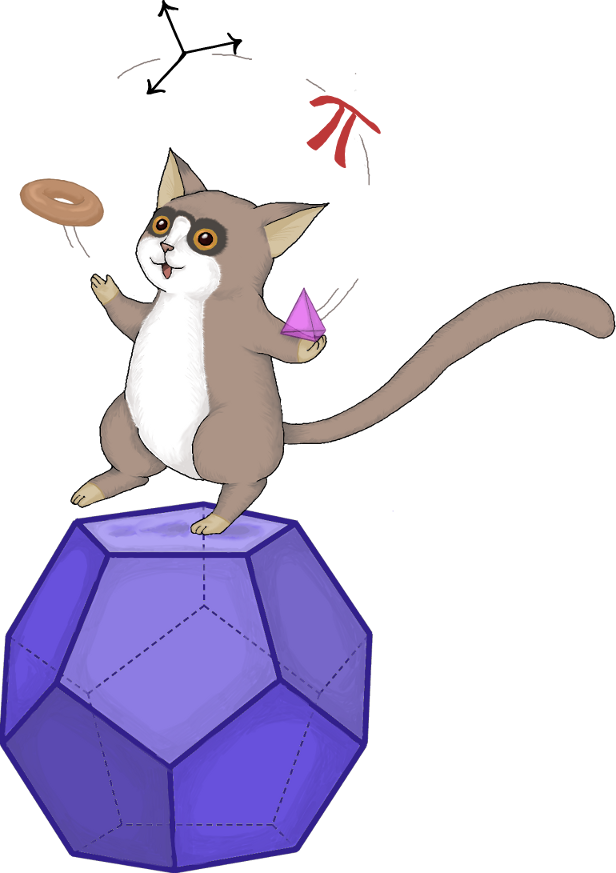
\includegraphics[scale=0.1]{cover}
%   }
%   \put(14.0,-3.5){%
%     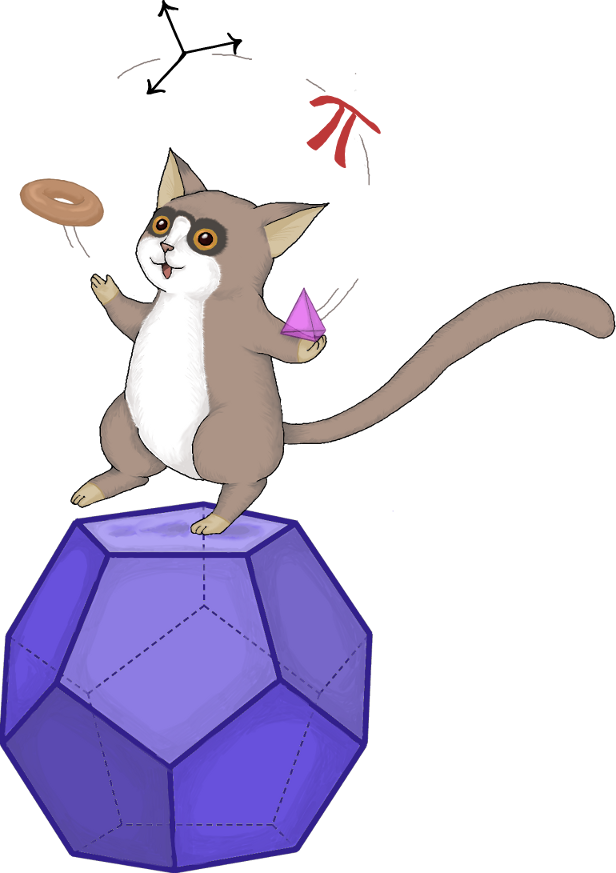
\includegraphics[scale=0.17]{cover}
%   }
% \end{picture} 

% \vspace{6em}
% \tableofcontents

% ab hier koennt ihr jetzt wirklich was machen

\maketitle{Gruppentheorie}{Dritter}

\tableofcontents


\section{Kurze Wiederholung von Gruppen}

Schon fr??h in der Schule lernt man, dass man mit Zahlen nicht nur Dinge abz??hlen kann, sondern auch rechnen kann. Doch was steckt eigentlich hinter der ganzen Struktur? Funktioniert das nur f??r Zahlen oder vielleicht auch f??r komplexere Dinge? Im letzten Jahr gab es einen Korrespondenzbrief, in dem ihr Gruppen und deren Wirkungen kennengelernt habt. Hier werden wir Gruppen noch ein wenig klassischer untersuchen und beginnen nochmal bei deren Definition sowie ersten Beispielen.

Zuerst verallgemeinern wir diese Operationen wie "`Plus"' und "`Mal"'. Sei $G$ eine beliebige Menge. Eine \textit{Verkn??pfung} $\circ$ ist eine Abbildung vom kartesischen Produkt $G\times G$ in die Menge $G$ selbst oder kurz geschrieben
\begin{equation*}
  \circ: G\times G \rightarrow G.
\end{equation*}
Das bedeutet, dass $\circ$ sich zwei Elemente aus der Menge $G$ nimmt und daraus ein neues macht. Genauso wie "`Plus"' und "`Mal"'.

\subsection{Die Definition einer Gruppe}

Ein Paar $(G??\circ )$ bestehend aus einer Menge $G$ und einer Verkn??pfung $\circ$ ist alleine noch nicht so spannend. Um von einer Gruppe zu reden, fordern wir folgende Eigenschaften, die ihr auch von "`Plus"' und "`Mal"' (bis auf eine Ausnahme) kennt.
\begin{itemize}
\item \textbf{A}ssoziativit??t: F??r je drei Elemente $a,b,c$ aus $G$ gilt $(a\circ b)\circ c = a\circ (b \circ c)$.
\item \textbf{N}eutrales Element: Es existiert ein Element $e$ in $G$, sodass f??r jedes andere Element $a$ aus $G$ $a\circ e = a = e\circ a$ gilt.
\item \textbf{I}nverses Element: Zu jedem Element $a$ aus $G$ existiert ein Element $a^{-1}$ in $G$, sodass $a\circ a^{-1} = e = a^{-1}\circ a$ gilt.
\end{itemize}
Erf??llt eine Gruppe zus??tzlich 
\begin{itemize}
\item \textbf{K}ommmutativit??t: F??r je zwei Elemente $a,b$ aus $G$ gilt $a\circ b = b\circ a$.
\end{itemize}
so nennt man sie \textbf{a}belsch.\footnote{Niels Henrik Abel, *05.08.1802, \textdagger 06.04.1829 war ein norwegischer Mathematiker. Bekannt ist er f??r abelsche Gruppen, abelsche Variet??ten und den Abel-Preis, der nach ihm benannt wurde. Er ist einer der wenigen Mathematiker, deren Namen als \emph{kleingeschriebene} Adjektive auch im Englischen ??blich sind.} Als kleine Eselsbr??cke dient dabei \textit{ANIKA}.

\subsection{Erste Beispiele}

Als erstes Beispiel w??ren da die ganzen Zahlen $\ZZ$ mit der Addition als Verkn??pfung. Das bedeutet f??r uns $a\circ b:=a+b$ mit $a,b\in\ZZ$.\footnote{Das Zeichen "`$:=$"' bedeutet eine Definition. Das hei??t, dass wir $a\circ b$ als $a+b$ definieren.} Diese Operation ist assoziativ (das lernt man sehr fr??h in der Schule), sie ist kommutativ (auch das kennt man aus der Schule) und es gibt ein neutrales Element, die Null. Das inverse Element zur ganzen Zahl $a$ ist die Zahl $-a$, denn $a+(-a)=0$. Damit haben alle ganzen Zahlen ein Inverses\footnote{Hier bedeutet "`Inverses"' invers bez??glich der Addition und \emph{nicht} bez??glich der Multiplikation. Die Bezeichnung $a^{-1}$ steht hier also f??r $-a$ und nicht $\frac{1}{a}$.} und $(\ZZ,+)$ bildet also eine Gruppe. 

\begin{aufgabe}{Gruppen-Check}
Untersuche folgende Paare auf ihre Gruppeneigenschaften. Falls vorhanden, wie sehen die neutralen Elemente und Inversen aus?
\begin{enumerate}
\item $(\mathbb{N}, +)$
\item $(\mathbb{Q}, +)$
\item $(\mathbb{R},\ \cdot\ )$
\item $(\mathbb{Q}\setminus \{0\},\ \cdot\ )$
\end{enumerate}
\end{aufgabe}

\subsection{Warum sind Gruppen wichtig?}

Ok, jetzt haben wir etwas, was wir schon gut kennen in eine Definition gepackt. Aber wozu das ganze? Das Interessante an Gruppen ist, dass diese sehr h??ufig in der Mathematik und der Physik auftreten, denn ganz oft hat man eine Verkn??pfung von Dingen, die die obigen Regeln erf??llt und dann kann man allgemeine Aussagen ??ber beliebige Gruppen verwenden.

Ein h??ufiger Ort, wo Gruppen auftauchen sind Probleme, in denen es eine "`Symmetrie"' gibt. Mit Symmetrie bezeichnen wir hier irgendeine Art von Transformation (zum Beispiel eine Bewegung), welche die Fragestellung oder gewissen Eigenschaften unver??ndert l??sst. Also ist zum Beispiel ein Kreis symmetrisch bez??glich Drehungen um den Mittelpunkt des Kreises. Allgemein lassen sich zwei solche Symmetrien hintereinander ausf??hren und man erh??lt eine neue Symmetrie. Beim Kreis sind zum Beispiel zwei Drehungen um den (orientierten) Winkel $\alpha$ eine Drehung um den Winkel $2\alpha$. Das inverse Element ist die Drehung um $-\alpha$ und das neutrale Element die Drehung, die nichts macht. Diese Symmetriegruppe ist sogar abelsch.

Symmetrien sind so grundlegend in der Physik, dass beispielsweise der Satz von Noether\footnote{} einer der wichtigsten in der theoretischen Physik ist. Anschaulich besagt er, dass das Vorhandensein von gewissen Symmetrien die Existenz einer Erhaltungsgr????e erzwingt. Alle Elementarteilchen im Standardmodell haben ihre Eigenschaften von gewissen Objekten, die man Gruppen zuordnet. Wenn Physiker also von elektromagnetischer Eichfeldtheorie sprechen, dann meinen sie, dass es eine Symmetriegruppe namens $U(1)$ gibt und diese legt fest, welche Arten von Elementarteilchen dieser Kraft entsprechen k??nnen.

\section{Weitere Beispiele}

Jetzt schauen wir uns mal etwas komplizierte Beispiele an.

\subsection{Symmetrische Gruppen}

Enorm wichtig in der Mathematik sind die \textit{symmetrischen Gruppen}. Zu jeder nat??rlichen Zahl $n\in \mathbb{N}$ gibt es eine symmetrische Gruppe $S_n$, deren Elemente angeben, wie man Zahlen von $1$ bis $n$ untereinander tauschen kann. Die Verkn??pfung von zwei Elementen ist eine Ausf??hrung der Vertauschungen nacheinander. Das erscheint im ersten Moment kompliziert, aber wir werden es anhand eines Beispiels vestehen.

Wir betrachten die $S_3$. Ein Element in der $S_3$ kann beispielsweise die Form 
\begin{equation*}
\begin{pmatrix}
 \textcolor{red}{1} & \textcolor{blue}{2} & \textcolor{green}{3} \\
 \textcolor{red}{2} & \textcolor{blue}{3} & \textcolor{green}{1}
\end{pmatrix}
\end{equation*}
haben. Dieses Element gibt folgende Vertauschung an: \textit{Die \textcolor{red}{1} wird auf die \textcolor{red}{2} geschickt, die \textcolor{blue}{2} wird auf die \textcolor{blue}{3} geschickt und die \textcolor{green}{3} wird auf die \textcolor{green}{1} geschickt}.

Bei der Verkn??pfung von zwei Elementen beginnt man zuerst mit dem rechten Element
\begin{equation*}
  \begin{pmatrix}
1 & 2 & 3 \\
2 & 3 & 1
  \end{pmatrix}
  \circ
  \begin{pmatrix}
1 & 2 & 3 \\
1 & 3 & 2
  \end{pmatrix}
  =
  \begin{pmatrix}
1 & 2 & 3 \\
a & b & c
  \end{pmatrix}.
\end{equation*}
Die Zahl $a$ erh??lten wir, indem wir uns ??berlegen auf welche Zahl die $1$ geschickt wird. Das rechte Element schickt $1$ auf $1$ und das linke Element die $1$ auf die $2$. Also ist $a=2$. Als n??chstes suchen wir $b$. Das rechte Element schickt die $2$ auf die $3$, das linke Element schickt die $3$ weiter auf die $1$. Also wird die $2$ insgesamt auf die $1$ geschickt, weshalb $b$ gleich $1$ ist. Somit bleibt f??r $c$ nur noch die $3$ ??brig. Damit erhalten wir
\begin{equation*}
  \begin{pmatrix}
1 & 2 & 3 \\
2 & 3 & 1
  \end{pmatrix}
  \circ
  \begin{pmatrix}
1 & 2 & 3 \\
1 & 3 & 2
  \end{pmatrix}
  =
  \begin{pmatrix}
1 & 2 & 3 \\
2 & 1 & 3
  \end{pmatrix}
\end{equation*}

\begin{aufgabe}{}
Finde alle sechs Elemente der $S_3$ und gib ihre Inversen an. Welches Element ist ??berhaupt das neutrale Element?
\end{aufgabe}

\begin{aufgabe}{}
Ist die $S_3$ eine kommutative Gruppe?
\end{aufgabe}

\begin{aufgabe}{}
Wieviele Elemente hat die $S_n$ f??r $n\in\NN$?
\end{aufgabe}


Jetzt kann man sich fragen, warum diese symmetrischen Gruppen ??berhaupt interessant sind. Eine Anwendung hat zum Beispiel die $S_{26}$. Ordnet man jedem Buchstaben ihre Stelle im Alphabet zu, so gibt ein Element der $S_{26}$ eine Vertauschung der Buchstaben an. Dies dient zur Verschl??sselung von Texten und ist deshalb so toll, weil man durch das inverse Element wieder zur??ck zum urspr??nglichen Text kommt. Sonderf??lle davon sind die \textit{Caesar\footnote{Gaius Iulius Caesar, *13.07. 100 v.Chr., \textdagger 15.03. 44 v.Chr., r??mischer Feldherr und Staatsmann, benutzte angeblisch die Caesar-Verschl??sselung f??r seine Truppen.}-Verschl??sselungen} oder auch die \textit{Vigen\`ere\footnote{Blaise de Vigen\`ere, *15.04.1523, \textdagger 1596, franz??sischer Diplomat und Kryptograf.}-Verschl??sselung}.

\subsection{Die W??rfelgruppe}

Ein weiteres Beispiel ist der Zauberw??rfel oder auch auf Englisch der "`Rubik's Cube"'. Fixieren wir seine sechs Seitenmittelpunkte, so kann man die restlichen 48 Fl??chen miteinander tauschen, indem man die Au??enseiten dreht.

Zun??chst ??berzeugen wir uns davon, dass die Drehungen der sechs Au??enseiten (die mittleren wollen wir fixieren, denn wir k??nnen ja immer den ganzen W??rfel zur??ck drehen) tats??chlich eine Gruppe bilden. Die Verkn??pfung ist das Hintereinanderausf??hren von zwei Z??gen, das neutrale Element macht einfach gar nichts und die Inversen sind gegeben durch das "`Zur??ckdrehen"'.

\begin{aufgabe}{}
  ??berzeuge dich davon, dass die W??rfelgruppe damit tats??chlich eine Gruppe ist. Ist die W??rfelgruppe kommutativ?
\end{aufgabe}

Insgesamt hat der W??rfel $9\times 6=54$ Teile, wobei wir die mittleren sechs fixieren wollen. Daher k??nnte man denken, dass wir mit den Drehungen diese Teile untereinander vertauschen k??nnen und damit die W??rfelgruppe die $S_{48}$ w??re. Allerdings kann man zum Beispiel Ecken mit Mittelst??cken nicht tauschen, weshalb wir hier nur eine Teilmenge der $S_{48}$ betrachten.

Aber das unglaubliche ist, dass wenn wir uns eine Tabelle rausschreiben mit allen m??glichen Zust??nden des W??rfels und ihnen die richtigen Elemente der $S_{48}$ zuordnen, wir direkt das Inverse bestimmen k??nnten, mit dem wir den W??rfel sofort l??sen k??nnen. Der einzige Haken dabei ist, dass die $S_n$ auch $n!$ viele Elemente besitzt und dies damit enorm schwierig und unpraktikabel w??re.

\subsection{Die Zopfgruppe}

Vielleicht habt ihr schonmal etwas von (mathematischen) Knoten geh??rt. Z??pfe sind so ??hnlich, bilden jedoch eine richtige Gruppe und haben dadurch gewisse Vorteile. Ihr Studium hilft auch beim Studium von Knoten. Daher schauen wir uns jetzt einmal diese Zopfgruppe an.

\subsubsection{Was sind Z??pfe?}

% Beispiele und Definition, insbesondere Herumziehen ist erlaubt

\begin{defn}
  Ein \emph{Zopf} auf $n$ Str??ngen ist ein Gebilde aus $n$ F??den, die sich nicht durchdringen d??rfen und sowohl oben als auch unten an $n$ Aufh??ngepunkten festgemacht sind. Au??erdem d??rfen die F??den immer nur nach unten gehen, also niemals wieder "`zur??ck nach oben"' gehen. Zwei Z??pfe sehen wir als gleich an, wenn man sie durch echte physikalische Bewegungen ineinander ??berf??hren kann, wobei man mit den F??den nicht ??ber das obere Ende oder unter das untere Ende gehen darf.\footnote{Nicht ganz un??berraschend ist die genaue mathematische Definition von "`F??den"' und "`physikalische Bewegung"'deutlich l??nger und nicht sehr spannend. Sie bedeutet genau das, was du denkst.}
\end{defn}

Einen Zopf illustrieren wir durch seine F??den. F??r die ??bersichtlichkeit f??rben wir manchmal die Str??nge ein. Zum Beispiel gilt 
\begin{equation*}
  \begin{aligned}
    \begin{tikzpicture}
      \braid  s_1 s_1^{-1};
    \end{tikzpicture}
  \end{aligned}
  =
  \begin{aligned}
    \begin{tikzpicture}
      \braid[number of strands={2}, yscale=5];
    \end{tikzpicture}
  \end{aligned}\; ,
\end{equation*}
wie man leicht einsieht.

Es gibt nun mehrere Fragen, die man sich stellen kann. Einerseits ben??tigt man f??r technische Argumente eine Art Baukasten aus Z??gen oder Bewegungen, die reichen um gleiche Z??pfe ineinander zu ??berf??hren. Analog wie bei Knoten sind dies die sogenannten Reidemeisterz??ge.

\begin{defn}
  Die \emph{Reidemeisterz??ge}\footnote{Kurt Werner Friedrich Reidemeister, *13.10.1893, \textdagger 08.07.1971, deutscher Mathematiker.} sind die folgenden Operationen:
  \begin{align*}
     \text{Typ II:}\qquad
    \begin{aligned}
    \begin{tikzpicture}
      \braid  s_1 s_1^{-1};
    \end{tikzpicture}
  \end{aligned}
  & =
  \begin{aligned}
    \begin{tikzpicture}
      \braid[number of strands={2}, yscale=5];
    \end{tikzpicture}
  \end{aligned}\; , \\
   \text{Type III:}\quad
  \begin{aligned}
    \begin{tikzpicture}
      \braid  s_1 s_2 s_1^{-1};
    \end{tikzpicture}
  \end{aligned}
  & =
  \begin{aligned}
    \begin{tikzpicture}
      \braid s_2^{-1} s_1 s_2;
    \end{tikzpicture}
  \end{aligned}\; , \\
  \end{align*}
\end{defn}

Es gibt daneben noch den Reidemeisterzug I, welcher eine kleine Schleife entdreht. Aufgrund der Definition von Z??pfen ben??tigen wir diesen Zug hier allerdings nicht. Den Reidemeisterzug III kann man sich vorstellen als das Vorbeiziehen eines Strangs hinter einer Kreuzung. Von allen Z??gen gibt es nat??rlich noch die gespiegelten Versionen, welche man auch als Reidemeisterz??ge bezeichnet.

Die Bedeutung dieser Z??ge liegt darin, dass man beweisen kann, dass sie ausreichen um gleiche Z??pfe zu identifizieren. Das hei??t, dass zwei Z??pfe gleich sind genau dann, wenn sie durch die endlich viele Reidemeisterz??ge sowie Verschiebungen von F??den, die nichts an den Kreuzungen ??ndern, ineinander ??berf??hren kann. 

% \begin{tikzpicture}
% \braid[style strands={1}{red}, style strands={2}{blue}, style strands ={3}{green}]  s_1 s_2 s_1^{-1};%s_1 s_2^{???1} s_1 s_2^{???1} s_1 s_2^{???1};
% \end{tikzpicture}

\subsubsection{Wie bilden Z??pfe eine Gruppe?}

Z??pfe mit gleich vielen Str??ngen, sagen wir $n$, bilden eine Gruppe $B_n$ indem man die Z??pfe hintereinander setzt. Beachte, dass dann die mittleren Verbindungspunkte nicht mehr am Ende oder Anfang sind und deswegen bewegt werden d??rfen. Zum Beispiel gilt

\begin{equation*}
  \begin{aligned}
    \begin{tikzpicture}
      \braid[style strands={1}{red}, style strands={2}{blue}]  s_1;
    \end{tikzpicture}
  \end{aligned}
  \circ
  \begin{aligned}
    \begin{tikzpicture}
      \braid[style strands={1}{blue}, style strands={2}{red}]  s_1^{-1};
    \end{tikzpicture}
  \end{aligned}
  =
  \begin{aligned}
    \begin{tikzpicture}
      \braid[style strands={1}{red}, style strands={2}{blue}]  s_1 s_1^{-1};
    \end{tikzpicture}
  \end{aligned}
  =
  \begin{aligned}
    \begin{tikzpicture}
      \braid[number of strands={2}, yscale=5, style strands={1}{red}, style strands={2}{blue}];
    \end{tikzpicture}
  \end{aligned}
\end{equation*}
Die H??he des Zopfes spielt dabei keine Rolle, es gibt also nur einen Zopf, der keinerlei Kreuzungen hat.

Das neutrale Element ist nun gegeben durch genau diesen Zopf ohne Kreuzungen, denn wenn wir ihn vor oder hinter einen beliebigen Zopf legen, dann wird dieser gar nicht ver??ndert.

Das inverse Element eines beliebigen Zopfes ist etwas schwieriger zu bestimmen. Dazu nutzen wir die Reidemeisterz??ge von oben. Aktzeptieren wir, dass die Reidemeisterz??ge ausreichen um gleiche Z??pfe zu identifizieren, so k??nnen wir folgende ??berlegung anstellen. Ein Zopf auf $n$ Str??ngen besteht aus Kreuzungen und nichts dazwischen. Das hei??t, wir k??nnen (bis auf Verschiebungen ohne Kreuzungen zu ver??ndern) jeden Zopf beschreiben durch eine Folge von Kreuzungen. Dann m??ssen wir jedoch beachten, dass zwei solche Abfolgen von Kreuzungen durchaus den gleichen Zopf beschreiben k??nnen.

Dies f??hrt auf die Idee der \emph{Pr??sentation} einer Gruppe. Einerseits geben wir sogenannte \emph{Erzeuger} an und andererseits fordern wir, dass diese gewisse \emph{Relationen} erf??llen. In unserem Fall sind die Erzeuger
\begin{align*}
  a_i  & =
   \begin{aligned}
    \begin{tikzpicture}
      \braid[number of strands={5}]  s_3 ;
    \end{tikzpicture}
  \end{aligned}\; , \\
  b_i & =
  \begin{aligned}
    \begin{tikzpicture}
      \braid[number of strands={5}]  s_3^{-1} ;
    \end{tikzpicture}
  \end{aligned} \\
\end{align*}
wobei der Index $i$ der Nummer des linken oberen Strangs entspricht. Das hei??t insbesondere, dass $i$ zwischen $1$ und $n-1$ eine beliebige nat??rliche Zahl sein kann. Die abgebildeten Z??pfe sind also konkret $a_3$ und $b_3$ in der $B_5$. Aus diesen Erzeugern k??nnen wir nun ein \emph{Wort}, das hei??t eine Kette von Erzeugern\footnote{??hnlich wie bei der Multiplikation von Zahlen l??sst man das Verkn??pfungszeichen oft weg.}, bilden. Zum Beispiel
\begin{equation*}
  a_1b_2a_1b_3a_2,
\end{equation*}
was dem folgenden Zopf in der Zopfgruppe $B_5$ auf $5$ Str??ngen\footnote{Beachte, dass also $a_1$ einen anderen Zopf in der $B_2$ entspricht als in der $B_5$.} entspricht
\begin{center}
  \begin{tikzpicture}
      \braid[number of strands={5}]  s_1 s_2^{-1} s_1 s_3^{-1} s_2;
    \end{tikzpicture} \; .
\end{center}
Ist dir anschaulich klar, dass man damit jeden Zopf beschreiben kann? Da aber die Reidemeisterz??ge gelten m??ssen, sind einige dieser W??rter gleich und wir beschreiben dies durch Gleichungen, die man Relationen nennt.

Reidemeisterzug I besagt zum Beispiel $a_ib_i=1$, also ist $b_i$ gerade das Inverse von $a_i$. Daher lassen wir die $b_i$'s von jetzt an weg und erlauben stattdessen $a_i^{-1}$ in unseren W??rtern. Reidemeisterzug II besagt nun die ber??hmte $ABA=BAB$-Relation
\begin{equation*}
  a_1a_2a_1=a_2a_1a_2,
\end{equation*}
welche f??r alle benachbarten Erzeuger $a_i$ und $a_{i+1}$ gilt. Als Diagramm bedeutet diese Gleichung
\begin{equation*}
  \begin{aligned}
    \begin{tikzpicture}
      \braid s_1 s_2 s_1;
    \end{tikzpicture}
  \end{aligned}
  =
  \begin{aligned}
    \begin{tikzpicture}
      \braid s_2 s_1 s_2;
    \end{tikzpicture}
  \end{aligned}\; ,
\end{equation*}
was offensichtlich stimmt.

\begin{aufgabe}{}
  Welche Relation erf??llen die Erzeuger $a_i$ und $a_j$, wenn der $i$-te und der $j$-te Strang nicht benachbart sind? Welches Diagramm entspricht dieser Aussage?
\end{aufgabe}

Damit haben wir den folgenden Satz verstanden:
\begin{satz}
  Die Zopfgruppe $B_n$ wird erzeugt von $a_1,\ldots,a_{n-1}$ mitsamt den Relationen $a_ia_{i+1}a_i=a_{i+1}a_ia_{i+1}$ f??r $i=1,\ldots,n-2$ und $a_ia_j=a_ja_i$ f??r $i,j=1,\ldots,n-1$ und $i=j\pm 1$.
\end{satz}

\subsubsection{Was haben Z??pfe mit Permutationen zu tun?}

% Kommutativit??t

% Gruppenhomomorphismen und Abbildung auf symmetrische Gruppen

Als erstes ??berlegen wir uns, wie die einfachsten Zopfgruppen eigentlich aussehen und ob diese abelsch sind.

\begin{aufgabe}{}
  Wie kann man die Zopfgruppe $B_1$ und die $B_2$ noch beschreiben? Welche Zopfgruppen sind kommutativ?
\end{aufgabe}

Jetzt schauen wir noch mal die Z??pfe selber an. Stellt euch vor, dass die Str??nge eines Zopfes oben nummeriert sind von $1$ bis $n$. Dann kann man den Z??pfen folgen und kommt unten an einem m??glicherweise anderen Strangende heraus, wenn man diese auch von $1$ bis $n$ nummeriert hat. Das hei??t, man kann aus einem Zopf eine Vertauschung beziehungsweise Permutation der Zahlen $1$ bis $n$ machen, also ein Element der symmerischen Gruppe auf $n$ Elementen, die wir ja schon oben gesehen haben. Schauen wir uns doch mal ein Beispiel an.

Der Zopf
\begin{center}
  \begin{tikzpicture}
      \braid[number of strands={5}]  s_1 s_2;
    \end{tikzpicture}
\end{center}
entspricht der Permutation
\begin{equation*}
  \begin{pmatrix}
    1 & 2 & 3 & 4 & 5 \\
    3 & 1 & 2 & 4 & 5
  \end{pmatrix}.
\end{equation*}

\begin{aufgabe}{}
  Stell dir vor, dass du zwei Z??pfe miteinander verkn??pfst, also untereinander verklebst. Sowohl die einzelnen Z??pfe als auch der neu entstandene Zopf entsprechen einer Permutation. Wie h??ngen diese Permutationen zusammen?
\label{aufgabe:zoepfe-perm}
\end{aufgabe}

Wenn ihr die letzte Aufgabe gel??st habt, dann seid ihr auf eines der wichtigsten Konzepte der Algebra oder eigentlich der gesamten Mathematik gesto??en, sogenannten \emph{Morphismen}. Hier handelt es sich um einen \emph{Homomorphismus}, was soviel bedeutet wie strukturerhaltende Abbildung.

\begin{defn}
  Seien $G$ und $H$ Gruppen. Dann hei??t eine Abbildung $\phi:G\lra H$ Gruppenhomomorphismus wenn
  \begin{equation*}
    \phi(g_1\circ g_2)=\phi(g_1)\circ\phi(g_2)
  \end{equation*}
  gilt f??r alle $g_1,g_2\in G$.
\end{defn}

Mit der Aufgabe~\ref{aufgabe:zoepfe-perm} habt ihr also gezeigt, dass die Abbildung
\begin{equation*}
  B_n\lra S_n,
\end{equation*}
die einem Zopf seine Vertauschung der Enden zuordnet ein Gruppenhomomorphismus ist.

\subsection{Nicht-Beispiele}

Bevor wir uns wieder allgemeinen Eigenschaften widmen, gibt es hier noch ein paar ausgefallenere Beispiele von Mengen und Verkn??pfungen, die \emph{keine} Gruppen bilden.

\subsubsection{Monoide}

Erinnert ihr euch noch an $ANIKA$? Als erstes wollen wir das $I$ weglassen, also eine Menge mit einer Verkn??pfung finden, die assoziativ ist und ein neutrales Element bestitzt, aber keine Inversen.\footnote{Das letzte $A$ stand ja f??r abelsche Gruppen, das interessiert uns jetzt einfach mal gar nicht.} So etwas nennt man \emph{Monoid}, insbesondere sind nicht alle Monoiden Gruppen.

Das einfachste Beispiel sind die nat??rlichen Zahlen (hier einfach mal inklusive Null) $0,1,2,3,\ldots$ mit der Addition. Die ist offensichtlich assoziativ und die Null erf??llt $a+0=a$, aber $1$ und $2$ und so weiter haben kein Inverses.

Ein anderes Beispiel w??ren die ganzen Zahlen mit der Multiplikation als Operation. Diese ist wieder assoziativ und es existiert ein neutrales Element -- die Eins -- aber au??er $1$ und $-1$ haben keine Zahlen ein Inverses.

\subsubsection{Nichtassoziative Mengen mit Verkn??pfungen und neutralem Element}

Jetzt betrachten wir einmal die ganzen Zahlen wie gewohnt -- aber mit der \emph{Subtraktion} als Gruppenoperation, also $a\circ b:=a-b$ f??r $a,b\in\ZZ$. Diese Operation hat ein neutrales Element und zwar die Null. Au??erdem hat jedes Element ein Inverses und zwar sich selbst, denn $a\circ a=a-a=0$. Aber die Operation ist nicht assoziativ, denn
\begin{align*}
  a\circ(b\circ c)&=a-(b-c)=a-b+c \\
  (a\circ b)\circ c&=(a-b)-c=a-b-c
\end{align*}
und die beiden rechten Seiten sind verschieden f??r $c\neq 0$. Damit verletzen wir das erste $A$ in $ANIKA$.

\section{Eigenschaften von Gruppen und Gruppenhomomorphismen}

Nat??rlich sind uns die Gruppenaxiome alleine nicht ausreichend. Aber damit k??nnen wir nun neue Eigenschaften direkt folgern.

%\subsection{Erste Eigenschaften}

Wir k??nnen beispielsweise zeigen, dass es in jeder Gruppe $(G,\circ)$ nur ein einziges neutrales Element gibt. Der Beweis dazu:

Angenommen es gibt zwei neutrale Elemente $e$ und $e^\prime$. Dann gilt
$$ e \stackrel{e^\prime\text{ ist}}{\stackrel{\text{neutral}}{=}} e\circ e^\prime \stackrel{e\text{ ist}}{\stackrel{\text{neutral}}{=}} e^\prime.$$

Jetzt sollst du als erstes einmal eine der wichtigsten Rechenregelen nachweisen, die wir auch so gewohnt sind von Zahlen.

\begin{aufgabe}{K??rzungsregeln}
Zeige folgende Aussage: Wenn f??r drei beliebige Elemente $a,b,c$ aus $G$ gilt $a\circ b = c\circ b$, dann folgt auch dass $a = c$ gilt.
\end{aufgabe}

In der Definition einer Gruppe haben wir nur vorrausgesetzt, dass ein inverses Element \emph{existiert}. Tats??chlich ist dieses aber auch eindeutig, wie die n??chste Aufgabe zeigt.

\begin{aufgabe}{Das Inverse Element ist eindeutig}
Zeige, dass zu jedem Element $a$ aus $G$ das inverse Element $a^{-1}$ eindeutig ist.
\end{aufgabe}

\begin{aufgabe}{Eigenschaften statt Gleichungen}
Zeige, dass f??r je zwei beliebige Elemente $a,b$ aus $G$ gilt $(a\circ b)^{-1} = b^{-1}\circ a^{-1}$.

\textit{Hinweis: Versuche nicht die Gleichung zu beweisen, sondern ??berlege dir, ob $b^{-1}\circ a^{-1}$ die Eigenschaft von $(a\circ b)^{-1}$  erf??llt und benutze eine fr??here Aufgabe.}
\end{aufgabe}

\begin{aufgabe}{Ordnungen und Kommutativit??t}
\begin{enumerate}
\item Beweise folgendes: Gilt f??r jedes Element $a$ aus $G$ dass $a\circ a = e$, so ist $(G,\circ)$ eine abelsche Gruppe (also kommutativ).
\item Gilt die Umkehrung des Satzes aus a)?
\item Kann der Satz aus a) wie folgt verallgemeinert werden: Gibt es eine nat??rliche Zahl $n$ derart, dass f??r jedes Element $a$ einer Gruppe  $a^n=e$ gilt\footnotemark, so ist die Gruppe kommutativ.
\end{enumerate}
\end{aufgabe}

\footnotetext{$a^n$ bedeutet hier $\overbrace{a\circ a\circ \cdots \circ a}^{n\text{ mal}}$.}

In der Definition eines Gruppenhomomorphismusses haben wir nur vorrausgesetzt, dass die Abbildung die Verkn??pfung erh??lt ($\phi(g_1\circ g_2)=\phi(g_1)\circ\phi(g_2)$). Eine Gruppe hat aber noch Inverse und ein neutrales Element. F??r die m??ssen wir jedoch nichs extra fordern, wie die n??chste Aufgabe zeigt

\begin{aufgabe}{Gruppenhomomorphismen}
  Beweise, dass f??r einen Gruppenhomomorphismus $\phi:G\lra H$ zwischen zwei Gruppen $G$ und $H$ gilt
  \begin{enumerate}
    \item $\phi(e_G)=e_H$, also dass $\phi$ das neutrale Element auf das neutrale Element abbildet und
    \item $\phi(g^{-1})=(\phi(g))^{-1}$ f??r alle $g\in G$.
  \end{enumerate}
\end{aufgabe}

% \subsection{Ordnungen und zyklische Gruppen}


\end{document}